\chapter{Reti Neurali Artificiali}
\begin{flushright}\small\textit{Lezione 10 -- 20/04/2026 -- G\'eron, Cap.\ 10}\end{flushright}

\section{Introduzione e applicazioni moderne}

Le \textbf{Reti Neurali Artificiali} (ANN -- \emph{Artificial Neural Networks}) sono modelli computazionali ispirati al funzionamento del cervello biologico. Sono alla base delle applicazioni più potenti dell'IA moderna:

\begin{itemize}
    \item \textbf{Visione artificiale}: riconoscimento di immagini, guida autonoma, diagnosi medica da immagini.
    \item \textbf{Linguaggio naturale}: traduzione automatica, chatbot, LLM (GPT, Claude).
    \item \textbf{Giochi}: AlphaGo e AlphaZero (DeepMind) hanno battuto i campioni mondiali di Go e scacchi.
    \item \textbf{Biologia}: AlphaFold ha predetto la struttura tridimensionale di quasi tutte le proteine conosciute.
    \item \textbf{Sistemi di raccomandazione}: Netflix, Spotify, Amazon.
    \item \textbf{Generative AI}: immagini (Stable Diffusion, DALL-E), testo, audio, video.
\end{itemize}

\begin{notebox}[Il problema del Cold Start]
Nei sistemi di raccomandazione, il \emph{Cold Start} è la difficoltà di suggerire prodotti a \textbf{nuovi utenti} (o nuovi prodotti) per mancanza di dati storici. Se un utente è nuovo, non ha acquistato nulla: su cosa si basa il sistema? Soluzioni: chiedere preferenze iniziali, usare feature di contenuto (genere, artista), dati demografici o embedding pre-addestrati.
\end{notebox}

\section{Dal neurone biologico al modello matematico}

Il cervello umano contiene circa $10^{11}$ neuroni, ciascuno connesso in media a $10^4$ altri neuroni. La comunicazione avviene attraverso impulsi elettrochimici (\emph{potenziali d'azione}).

\begin{center}
\begin{tikzpicture}[font=\footnotesize]
\node[circle, draw=MidnightBlue, fill=blue!8, very thick,
      minimum size=1.4cm, align=center] (soma) at (5, 0) {Soma\\(nucleo)};
\foreach \i/\y/\lbl in {1/2.0/{$x_1$, peso $w_1$},
                          2/0.7/{$x_2$, peso $w_2$},
                          3/-0.7/{$x_3$, peso $w_3$},
                          4/-2.0/{$x_4$, peso $w_4$}} {
    \draw[very thick, MidnightBlue, -{Stealth[length=2.5mm]}]
        (1.5, \y) -- (soma.west);
    \node[anchor=east, font=\scriptsize] at (1.5, \y) {\lbl};
    \node[anchor=east, font=\scriptsize, gray] at (-0.5, \y) {dendrite \i};
}
\draw[very thick, BrickRed, -{Stealth[length=2.5mm]}]
    (soma.east) -- node[above, font=\scriptsize] {assone (output)} (9, 0);
\node[anchor=west, font=\scriptsize] at (9, 0) {output $\hat{y}$};
\node[font=\scriptsize, OliveGreen, align=center] at (5, -1.4)
    {$z = \sum w_i x_i + b$\\$\hat{y} = f(z)$};
\end{tikzpicture}
\end{center}

\begin{itemize}
    \item \textbf{Dendriti} (input): ricevono i segnali dalle sinapsi -- corrispondono alle feature $x_i$.
    \item \textbf{Soma} (elaborazione): calcola la somma pesata dei segnali in ingresso.
    \item \textbf{Assone} (output): trasmette il segnale se supera una soglia -- corrisponde all'output $\hat{y}$.
    \item \textbf{Pesi sinaptici} $w_i$: la forza della connessione tra due neuroni. Idea di Hebb (1949): \emph{``Neurons that fire together wire together''} -- i neuroni che si attivano insieme rinforzano il loro legame.
\end{itemize}

\subsection{McCulloch \& Pitts (1943)}

Il primo modello formale di neurone artificiale: input e output binari (0/1), soglia fissa. Dimostrarono che una rete finita di tali neuroni può calcolare qualsiasi \textbf{funzione booleana} -- AND, OR, NOT e le loro combinazioni.

\begin{exbox}[Calcoli logici con i neuroni]
Si possono costruire le porte logiche fondamentali con neuroni a soglia. La soglia scatta quando $z \geq \theta$:

\textbf{AND} (2 input): pesi $w_1 = w_2 = 1$, soglia $\theta = 2$. Output 1 solo se \emph{entrambi} gli input sono 1: $z = 1+1 = 2 \geq 2$ {\checkmark}.

\textbf{OR} (2 input): pesi $w_1 = w_2 = 1$, soglia $\theta = 1$. Output 1 se \emph{almeno uno} è 1: $z = 1 \geq 1$ {\checkmark}.

\textbf{NOT} (1 input): peso $w_1 = -1$, bias $b = 1$. Output 1 se input è 0: $z = -0 + 1 = 1 \geq 1$ {\checkmark}.

Combinando AND, OR e NOT è possibile costruire qualsiasi circuito logico -- in teoria, un cervello artificiale.
\end{exbox}

\section{Il Percettrone}

Frank Rosenblatt (1957) generalizza il neurone McCulloch-Pitts introducendo i \textbf{pesi apprendibili}: anziché fissare $w_i$ manualmente, il percettrone li impara dai dati.

\subsection{Matematica del percettrone}

\begin{equation}
z = w_1 x_1 + w_2 x_2 + \dots + w_n x_n + b = \mathbf{w}^T \mathbf{x} + b
\end{equation}

\begin{notebox}[Perché la trasposta $\mathbf{w}^T$?]
Per convenzione $\mathbf{w}$ e $\mathbf{x}$ sono vettori colonna. Il prodotto scalare si calcola moltiplicando riga per colonna, quindi si traspone il vettore pesi: $\mathbf{w}^T \mathbf{x} = \sum_i w_i x_i$. È solo notazione -- il risultato è lo stesso.
\end{notebox}

\subsection{Funzione di attivazione Heaviside}

Il percettrone classico usa la \textbf{funzione gradino di Heaviside}:

\begin{equation}
H(z) =
\begin{cases}
0 & \text{se } z < 0 \\
1 & \text{se } z \geq 0
\end{cases}
\end{equation}

L'output è binario: il neurone \emph{spara} (1) se il segnale totale supera la soglia, altrimenti rimane silenzioso (0).

\begin{exbox}[Analogia sensoriale]
\textbf{Udito in un bar affollato}: il rumore di fondo costante non supera la soglia neuronale -- viene filtrato. Se qualcuno urla il tuo nome, il peso $w_i$ associato al suono del tuo nome è alto: $z \geq 0$ e il neurone ``spara'', facendoti girare la testa.

\textbf{Vista}: una luce ambiente costante non attiva i fotorecettori di risposta al movimento. Una luce stroboscopica sì -- è il cambiamento rapido che supera la soglia.
\end{exbox}

\subsection{Regola di apprendimento di Hebb}

Il percettrone aggiorna i pesi in base all'errore -- quanto la previsione si discosta dal target reale:

\begin{equation}
\boxed{w_{i}^{(\text{next})} = w_{i} + \eta \cdot (y - \hat{y}) \cdot x_i}
\end{equation}

dove $\eta$ è il \textbf{learning rate} (tasso di apprendimento) -- un iperparametro che controlla quanto è grande ogni aggiornamento.

\begin{itemize}
    \item Se $\hat{y} = y$ (previsione corretta): errore $= 0$, nessun aggiornamento.
    \item Se $\hat{y} < y$ (sotto-stima): i pesi per gli input positivi aumentano.
    \item Se $\hat{y} > y$ (sovra-stima): i pesi per gli input positivi diminuiscono.
\end{itemize}

\textbf{Teorema di convergenza di Rosenblatt (1958)}: se i dati sono \textbf{linearmente separabili}, l'algoritmo converge in un numero finito di passi -- troverà sempre una soluzione.

\subsection{Limiti del percettrone e l'Inverno dell'IA}

Il percettrone classico risolve solo problemi \textbf{linearmente separabili} -- quelli in cui esiste una retta (o un iperpiano) che separa le due classi.

\begin{warnbox}[Il problema dello XOR]
Nel libro \emph{Perceptrons} (1969), Minsky e Papert dimostrarono che un singolo percettrone \textbf{non può} risolvere la funzione XOR: le classi $\{(0,0),(1,1)\}$ (output 0) e $\{(0,1),(1,0)\}$ (output 1) non sono separabili da nessuna retta.

Questo risultato -- amplificato oltre misura -- causò il \textbf{Primo Inverno dell'IA}: finanziamenti tagliati, interesse crollato, ricerca bloccata per un decennio.
\end{warnbox}

\begin{center}
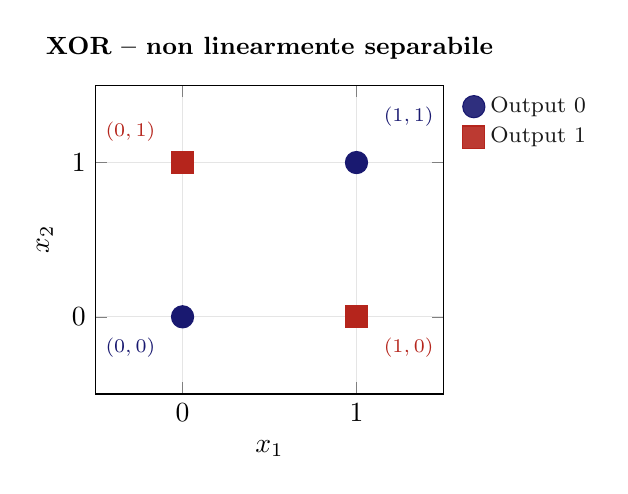
\begin{tikzpicture}
\begin{axis}[
    width=6cm, height=5.5cm,
    xlabel={$x_1$}, ylabel={$x_2$},
    xmin=-0.5, xmax=1.5, ymin=-0.5, ymax=1.5,
    xtick={0,1}, ytick={0,1},
    grid=major, grid style={gray!20},
    title={\small XOR -- non linearmente separabile},
    title style={font=\small\bfseries},
    legend pos=outer north east,
    legend style={font=\footnotesize, cells={anchor=west},
                  legend columns=1, draw=none, fill=white, fill opacity=0.9},
    legend cell align={left},
    clip=false
]
\addplot[only marks, mark=*, mark size=4pt, MidnightBlue]
    coordinates {(0,0)(1,1)};
\addlegendentry{Output 0}
\addplot[only marks, mark=square*, mark size=4pt, BrickRed]
    coordinates {(0,1)(1,0)};
\addlegendentry{Output 1}
\node[font=\scriptsize, MidnightBlue] at (axis cs:-0.3, -0.2) {$(0,0)$};
\node[font=\scriptsize, MidnightBlue] at (axis cs:1.3, 1.3) {$(1,1)$};
\node[font=\scriptsize, BrickRed] at (axis cs:-0.3, 1.2) {$(0,1)$};
\node[font=\scriptsize, BrickRed] at (axis cs:1.3, -0.2) {$(1,0)$};
\end{axis}
\end{tikzpicture}
\end{center}

La soluzione è aggiungere \textbf{strati nascosti} -- i \emph{Multi-Layer Perceptron} possono risolvere XOR e qualsiasi altra funzione.

\section{Architettura del Multi-Layer Perceptron (MLP)}

Un \textbf{MLP} è una rete feed-forward (il segnale fluisce solo in avanti) con uno o più \textbf{hidden layer} tra input e output.

\begin{center}
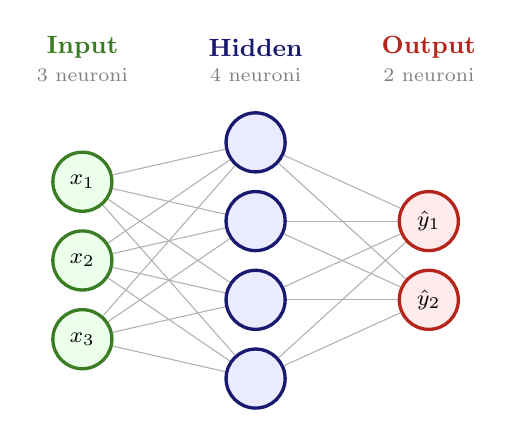
\begin{tikzpicture}[font=\footnotesize, x=2.2cm, y=1.0cm,
    inp/.style={circle, draw=OliveGreen, fill=green!8, very thick,
                minimum size=0.75cm, inner sep=0pt},
    hid/.style={circle, draw=MidnightBlue, fill=blue!8, very thick,
                minimum size=0.75cm, inner sep=0pt},
    outn/.style={circle, draw=BrickRed, fill=red!8, very thick,
                minimum size=0.75cm, inner sep=0pt}
]
\foreach \i/\lbl in {1/$x_1$, 2/$x_2$, 3/$x_3$}
    \node[inp] (i\i) at (0, -\i+0.5) {\lbl};
\foreach \j in {1,2,3,4}
    \node[hid] (h\j) at (1, -\j+1.0) {};
\foreach \k/\lbl in {1/$\hat{y}_1$, 2/$\hat{y}_2$}
    \node[outn] (o\k) at (2, -\k+0.0) {\lbl};
\foreach \i in {1,2,3}
    \foreach \j in {1,2,3,4}
        \draw[gray!60, thin] (i\i) -- (h\j);
\foreach \j in {1,2,3,4}
    \foreach \k in {1,2}
        \draw[gray!60, thin] (h\j) -- (o\k);
\node[font=\small\bfseries, OliveGreen] at (0, 1.2) {Input};
\node[font=\scriptsize, gray] at (0, 0.85) {3 neuroni};
\node[font=\small\bfseries, MidnightBlue] at (1, 1.2) {Hidden};
\node[font=\scriptsize, gray] at (1, 0.85) {4 neuroni};
\node[font=\small\bfseries, BrickRed] at (2, 1.2) {Output};
\node[font=\scriptsize, gray] at (2, 0.85) {2 neuroni};
\end{tikzpicture}
\end{center}

\textbf{Dense Layer} (o \emph{Fully Connected}): ogni neurone è connesso a \emph{tutti} i neuroni dello strato precedente. In forma matriciale:
\[
\mathbf{Z} = \mathbf{X} \mathbf{W} + \mathbf{b}
\qquad
\mathbf{X} \in \mathbb{R}^{m \times n}, \quad \mathbf{W} \in \mathbb{R}^{n \times h}, \quad \mathbf{b} \in \mathbb{R}^{h}
\]

\begin{notebox}[Perché GPU e TPU?]
Il calcolo dei layer densi si riduce a moltiplicazioni matriciali -- operazioni altamente parallelizzabili. Le GPU (originalmente progettate per rendering 3D) e le TPU (Tensor Processing Units, Google) eseguono migliaia di queste operazioni contemporaneamente: una rete che su CPU richiederebbe ore si addestra in minuti.

Al contrario, algoritmi \emph{sequenziali} come il calcolo di Fibonacci (ogni passo dipende dai due precedenti) non beneficiano della parallelizzazione.
\end{notebox}

\section{Funzioni di attivazione}

Senza funzioni di attivazione non lineari, un MLP con più layer sarebbe equivalente a un singolo layer lineare -- inutile. Le funzioni di attivazione \textbf{introducono la non-linearità} che permette alla rete di approssimare funzioni complesse.

\begin{center}
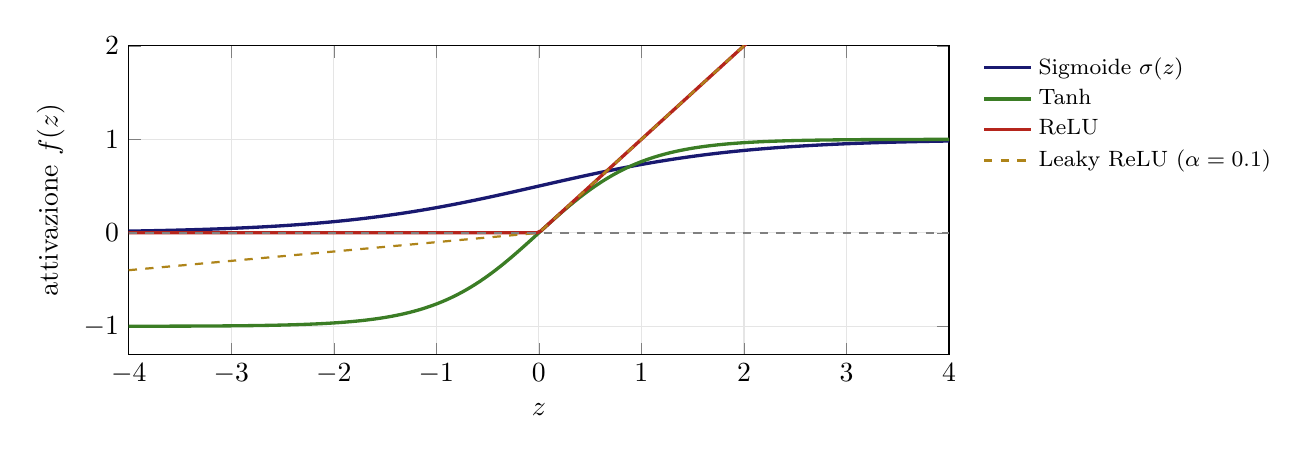
\begin{tikzpicture}
\begin{axis}[
    width=12cm, height=5.5cm,
    xlabel={$z$}, ylabel={attivazione $f(z)$},
    xmin=-4, xmax=4, ymin=-1.3, ymax=2.0,
    grid=major, grid style={gray!20},
    legend pos=outer north east,
    legend style={font=\footnotesize, cells={anchor=west},
                  legend columns=1, draw=none}
]
\addplot[domain=-4:4, samples=200, very thick, MidnightBlue]
    {1/(1+exp(-x))};
\addlegendentry{Sigmoide $\sigma(z)$}
\addplot[domain=-4:4, samples=200, very thick, OliveGreen]
    {tanh(x)};
\addlegendentry{Tanh}
\addplot[domain=-4:4, samples=200, very thick, BrickRed]
    {max(0,x)};
\addlegendentry{ReLU}
\addplot[domain=-4:4, samples=200, thick, Goldenrod!80!black, dashed]
    {(x > 0) ? x : 0.1*x};
\addlegendentry{Leaky ReLU ($\alpha=0.1$)}
\addplot[thick, gray, dashed] coordinates {(-4,0)(4,0)};
\end{axis}
\end{tikzpicture}
\end{center}

\begin{itemize}
    \item \textbf{Sigmoide} $\sigma(z) = \frac{1}{1+e^{-z}}$: output in $(0,1)$. Utile nell'output per classificazione binaria. Problema: \textbf{saturazione} -- per $z$ molto grandi o piccoli, il gradiente tende a zero (\emph{vanishing gradient}).
    \item \textbf{Tanh}: output in $(-1,1)$, centrata in zero -- convergenza più veloce della sigmoide. Stesso problema di saturazione.
    \item \textbf{ReLU} $\max(0, z)$: standard de facto per i layer nascosti. Veloce da calcolare, nessuna saturazione per $z > 0$. Problema: \emph{dying ReLU} -- neuroni con $z < 0$ hanno gradiente sempre zero e smettono di imparare.
    \item \textbf{Leaky ReLU}: $\max(\alpha z, z)$ con $\alpha$ piccolo (es.\ 0.1). Risolve il dying ReLU mantenendo un piccolo gradiente per $z < 0$.
\end{itemize}

\section{Backpropagation}

L'algoritmo \textbf{backpropagation} (Rumelhart, Hinton, Williams 1986) è il motore dell'addestramento delle reti neurali: calcola efficientemente il gradiente della funzione di costo $L$ rispetto a \emph{tutti} i pesi.

\subsection{Le quattro fasi}

\begin{enumerate}
    \item \textbf{Forward pass}: un mini-batch di dati attraversa la rete strato per strato; si calcolano tutte le attivazioni $\mathbf{a}^{(l)}$ e infine l'output $\hat{\mathbf{y}}$.
    \item \textbf{Calcolo della loss}: si confronta $\hat{\mathbf{y}}$ con il target $\mathbf{y}$ tramite la funzione di costo (es.\ MSE, Cross-Entropy).
    \item \textbf{Backward pass}: si applica la \textbf{regola della catena} a ritroso, propagando il gradiente da output a input:
    \[
    \frac{\partial L}{\partial w_{ij}^{(l)}} = \delta_j^{(l)} \cdot a_i^{(l-1)}
    \]
    dove $\delta_j^{(l)}$ è il ``segnale di errore'' del neurone $j$ al layer $l$.
    \item \textbf{Aggiornamento dei pesi} con gradient descent:
    \[
    \mathbf{w} \leftarrow \mathbf{w} - \eta \, \nabla_{\mathbf{w}} L
    \]
\end{enumerate}

\begin{notebox}[Backpropagation non è magia]
La backpropagation è semplicemente una \textbf{applicazione efficiente della regola della catena} del calcolo differenziale. Il nome ``back'' viene dal fatto che i gradienti fluiscono all'indietro -- dall'output all'input -- mentre i dati nel forward pass fluiscono in avanti. L'efficienza viene dal riutilizzare i calcoli intermedi già fatti nel forward pass.
\end{notebox}

\section{Regressione e classificazione con MLP}

L'output layer si configura in base al tipo di problema. Tutto il resto della rete (layer nascosti) usa tipicamente ReLU.

\begin{center}
\renewcommand{\arraystretch}{1.4}
\begin{tabular}{@{} l p{3.8cm} p{5.2cm} @{}}
\toprule
\textbf{Problema} & \textbf{Output layer} & \textbf{Funzione di costo} \\
\midrule
Regressione (1 valore) & 1 neurone lineare & MSE o Huber loss \\
Regressione ($K$ valori) & $K$ neuroni lineari & MSE / Huber \\
Classificazione binaria & 1 neurone + Sigmoide & Binary Cross-Entropy \\
Classificazione multilabel & $K$ neuroni + Sigmoide & Binary Cross-Entropy \\
Classificazione multiclasse & $K$ neuroni + \textbf{Softmax} & Categorical Cross-Entropy \\
\bottomrule
\end{tabular}
\end{center}

\begin{defbox}[Softmax]
La funzione \textbf{Softmax} trasforma un vettore di logit (punteggi grezzi) in una distribuzione di probabilità:
\[
\text{softmax}(\mathbf{z})_k = \frac{e^{z_k}}{\displaystyle\sum_{j=1}^{K} e^{z_j}}, \qquad \sum_{k=1}^{K} \text{softmax}(\mathbf{z})_k = 1
\]
Usata nell'output layer multiclasse: garantisce che le probabilità siano tutte positive e sommino a 1. La classe predetta è quella con probabilità massima.
\end{defbox}

\begin{exbox}[Classificazione su MNIST con Keras]
La rete ha $784 \times 300 + 300 = 235\,500$ parametri nel primo layer, $300 \times 100 + 100 = 30\,100$ nel secondo, $100 \times 10 + 10 = 1\,010$ nel terzo -- totale $\approx 267\,000$ parametri addestrabili.
\end{exbox}

\section{Fine-tuning degli iperparametri}

Un MLP ha molti iperparametri da scegliere. Géron suggerisce alcune regole pratiche:

\begin{itemize}
    \item \textbf{Numero di layer nascosti}: iniziare con 1--2 layer (sufficienti per la maggior parte dei problemi). Aggiungere profondità solo se il modello è insufficiente -- le reti profonde imparano gerarchie di feature (bordi $\to$ texture $\to$ parti $\to$ oggetti).
    \item \textbf{Numero di neuroni per layer}: tipicamente tra 32 e 512, potenze di 2 per compatibilità GPU. Conviene iniziare largo e poi ridurre.
    \item \textbf{Learning rate $\eta$}: l'iperparametro più importante da sintonizzare. Troppo alto: instabilità. Troppo basso: convergenza lentissima. Valore tipico: $10^{-3}$ con Adam.
    \item \textbf{Batch size}: 32--256. Batch grandi convergono più velocemente ma generalizzano peggio.
    \item \textbf{Ottimizzatore}: Adam è il default moderno (adatta automaticamente il learning rate per ogni parametro).
\end{itemize}

\textbf{Metodi di ricerca degli iperparametri}:
\begin{itemize}
    \item \textbf{Grid search}: prova ogni combinazione di una griglia predefinita. Esaustivo ma costoso.
    \item \textbf{Random search}: campiona combinazioni casuali -- spesso più efficiente della grid search.
    \item \textbf{Bayesian optimization}: usa un modello probabilistico per guidare la ricerca (Optuna, Keras Tuner, Hyperopt).
\end{itemize}

\section{Teorema di approssimazione universale}

\begin{thmbox}[Cybenko (1989) -- Hornik (1991)]
Un MLP con un \textbf{singolo hidden layer} di larghezza sufficiente e funzione di attivazione non polinomiale può approssimare qualsiasi funzione continua su un insieme compatto, con precisione arbitraria.
\end{thmbox}

In altre parole: in teoria, una rete neurale può imparare \emph{qualsiasi cosa}. In pratica, però:

\begin{itemize}
    \item Reti \textbf{profonde} (molti layer) sono più efficienti delle reti \textbf{larghe} (un solo layer enorme): imparano gerarchie di feature con meno parametri totali.
    \item Più profondità $\to$ nuovi problemi: \textbf{vanishing gradient} e training instabile. Questo è l'argomento della prossima lezione.
\end{itemize}